\section{Random Forest}
The last classifier used is the \class{RandomForestClassifier()} from \code{sklearn.ensemble}.
A random forest is a type of ensemble learning method.
An ensemble method is a machine learning technique that combines the predictions of multiple models to make more accurate predictions than any individual model.
In a Random Forest, a set of decision trees are typically trained on a subset of the original dataset, however in some cases each tree can be trained on the entire data set.
The predicted class of an input sample is a vote by the trees in the forest, weighted by their probability estimates.
That is, the predicted class is the one with highest mean probability estimate across the trees.
This means that a random forest is not as prone to overfitting as a single decision tree, since this voting process helps to reduce the variance of the model.

\begin{figure}[H]
    \centering
    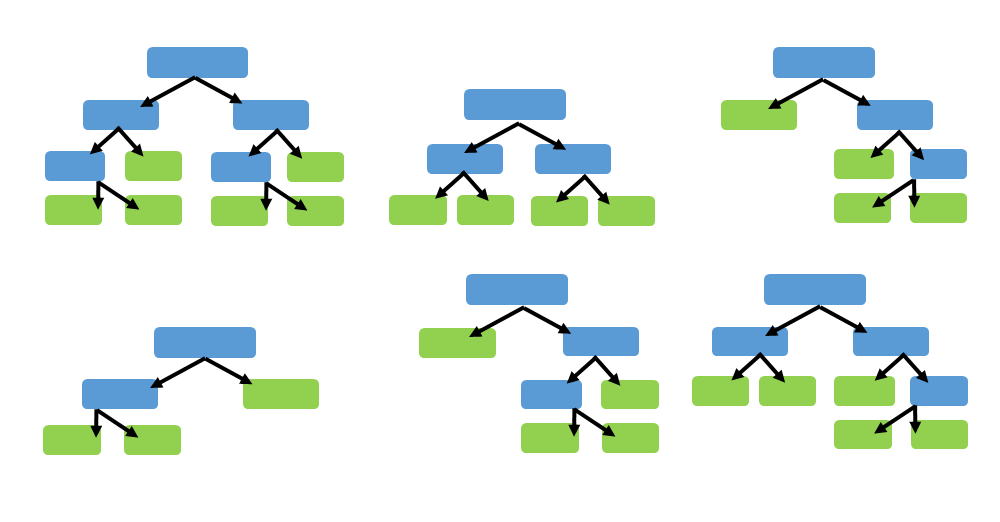
\includegraphics[scale=0.3]{figures_for_report/random_forest_simple_example}
    \captionsetup{justification=centering,margin=2cm}
    \caption{Random forest illustration}\label{fig:figure}
\end{figure}


\subsection{Hyperparameters}\label{subsec:hyperparameters}
The hyperparameters was chosen similar to the \class{DecisionTreeClassifier()}.
One additional parameter was looked at, \code{bootstrap}.
Boostrap refers to whether to use the entire dataset or sample from when building the trees.
The parameter grid used was the following:\\

\begin{center}
    \begin{minipage}{4in}
\begin{itemize}
    \item \code{max_depth}: [None, 10, 15, 20, 21, 22, 23]
    \item \code{min_samples_split}: [2, 4, 8]
    \item \code{criterion}: [gini, entropy]
    \item \code{bootstrap}: [True, False] \\
\end{itemize}
            \end{minipage}
\end{center}

which gave the best combination as:\\

\begin{tcolorbox}[colback=white,
                  arc=0pt,
                outer=0pt]
\centering \code{max_depth=21} \, \, \code{min_samples_split=4} \, \, \code{criterion=gini} \, \, \code{boostrap=False}\\
   \end{tcolorbox}


Using the entire dataset did not cause overfitting for this particular dataset, so \code{boostrap} was set to false.
These values were selected due to their ability to effectively prevent overfitting and improve the accuracy of the model, just like the decision tree parameters.
Then an instance of the \class{RandomForestClassifier()} was trained, with the parameters, while keeping all others at their default values.
Additionally \code{random_state=42} was again used, and will lead to the reproduction of the results reported in the next section.

\subsection{Results}\label{subsec:results}
\begin{table}[!ht]
\begin{subtable}[c]{0.4\textwidth}
\footnotesize
\centering
\begin{tabular}{ c | c }
 \toprule
 Evaluation Metric & Accuracy Score  \\
 \midrule
 Training Accuracy &  100\% \\
 Test Accuracy &85.54\% \\
 \bottomrule
\end{tabular}
\captionsetup{justification=centering,margin=1cm}
\end{subtable}
\begin{subtable}[c]{0.6\textwidth}
\footnotesize
\centering
\begin{tabular}{c | c c r}
Class & Precision & Recall & F1-Score\\
\midrule
T-shirt/Top   &    0.82  &    0.86  &    0.84 \\
Trousers   &    0.99  &    0.96  &    0.97 \\
Pullover   &    0.83  &    0.89  &    0.86\\
Dress   &    0.89  &    0.93  &    0.91\\
Shirt   &    0.74  &    0.64  &    0.69\\
\end{tabular}
\captionsetup{justification=centering,margin=1cm}
\end{subtable}
\caption{Random Forest Performance}
\label{tab:random_forest_evaluation}
\end{table}\\

\subsection{Discussing Results}